\section*{Βήμα 9}

Πρώτα από όλα κάνουμε clone τα δεδομένα σε μορφή .wav από το repository της εργασίας στον υπολογιστή μας. \\

\noindent Στη συνέχεια, αξιοποιύμε τον βοηθητικό κώδικα του εργαστηρίου προκειμένου να υλοποιήσουμε τα επόμενα βήματά μας (\textit{parser.py, hmm.py})

\lstinputlisting[language=Python, firstline=138, lastline=162]{../../lab.py}

\noindent Όπως φαίνεται και στη συνάρτηση παραπάνω, διαβάζουμε από το φάκελο τα wav αρχεία και εξάγουμε 13 MFCC για το καθένα. Στη συνέχεια με την έτοιμη συνάρτηση split του κώδικα τη χωρίζουμε στο default train test split το οποίο έχει 2700 από τα 3000 δείγματα ακολουθιών στο train και τα υπόλοιπα στο test. Στη συνέχεια, καλούμαστε να χωρίσουμε το test set αυτό σε 2 μικρότερα. Ένα validation και ένα test set σε αναλογία 80-20 αντίστοιχα. Αυτό, όπως φαίνεται και στον κώδικα παραπάνω, γίνεται με τη χρήση του \textit{train\_test\_split}. Η παράμετρος stratify μας εξασφαλίζει την ομοιόμορφη κατανομή των δειγμάτων. Δηλαδή, ότι θα έχουμε τον ίδιο αριθμό ψηφίων από κάθε κατηγορία. Έτσι αποφεύγουμε biases.

\begin{figure}[H]
	\centering
	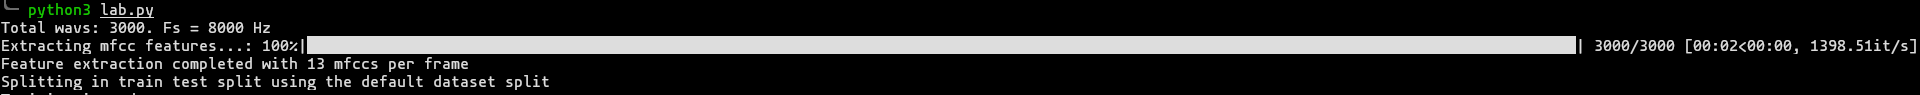
\includegraphics[width=\linewidth]{images/step9.png}
	\caption{Ανάγνωση Dataset}
\end{figure}


